\cleardoublepage%
\chapter{\label{chap:res}Results and discussion}%

This is where you present your findings. As much as possible, structure your results along the lines of your research questions. Start with the simplest results first and proceed to more complex ones. Tables and Figures should be clear enough that they need little explanation: do not simply re-write the numbers as text to fill space. Rather, highlight trends, outliers, or gaps. 

\section{\label{sec:res_disc}Discussion}

Sometimes, the discussion section is separate from the results. Where to include it is personal, though it is often easier to include the discussion with the results. The discussion simply refers to the interpretation and contextualization of the results.

You present your findings (results) and then explain what they mean;  how they relate to what other people have found;  how they match or contradict the literature. The discussion requires references to other published works. Results sections that only present data are fine, but when there are multiple results, it is sometimes difficult for the reader to bounce back and forth between the results and the discussion.

\section{\label{sec:res_tab_fig_math}Tables, Figures, and Mathematics}

Tables and Figures are key to communicating your results, so they need to be clear, organized, and well-presented. \textbf{Both Tables and Figures have to always be referenced in text}. They should be referenced on the same page as they appear, in the worst case, they can be referenced on the adjacent page of the two-page document, so the reader does not need to flip five pages to find the desired figure/table. The above rule applies to the first reference of figure/table in text. You can refer to the tables and figures, you have shown earlier, as many times as you reasonably need.

\subsection{\label{sec:res_tab}Tables}

Tables are numerical values or text displayed in rows and columns. When appearing in a document, tables should be numbered and appear sequentially. \textbf{Tables MUST always be referred to in text. They must be referred to by their number; the same applies to figures}. It is not appropriate to ask a reader to refer to a Table “above” or “below” as printing, screens, and downloads may all modify the location. \textbf{The table title ALWAYS appears at the top}. If there is not enough space on a page for a full table, move it. Actually, latex should do it for you. Only split the table between multiple pages if it is very long. Do not force your reader to flip back and forth in an effort to remember what the column headings are, the proper formatting of a long table (with the \texttt{longtable} package) should help keeping the headings organized on multiple pages. For an example of a well-formatted Table, see Table~\ref{tab:waste_gen}. 

\begin{table}
  \begin{center}
    \caption{\label{tab:waste_gen}Waste generation and collection in urban area of Africa for the year 2012}
    \begin{tabular}{lcccc}
      \toprule
        Region & Generation                 & Generation            & Collection            & \% collected \\
               & ${\rm kg~/~(capita~year)}$ & ${\rm 10^6~t~/~year}$ & ${\rm 10^6~t~/~year}$ & -            \\
        \midrule
        Eastern Africa     & 185.73 & 12.86 & 4.92  & 38.25 \\
        Western Africa     & 175.37 & 27.02 & 10.66 & 39.45 \\
        Central Africa     & 194.57 & 11.09 & 4.83  & 40.56 \\
        Southern Africa    & 247.00 & 26.34 & 13.05 & 49.54 \\
        Northern Africa    & 441.80 & 43.95 & 32.27 & 73.41 \\
        Sub-Saharan Africa & 200.67 & 78.12 & 33.46 & 42.83 \\
        \bottomrule
    \end{tabular}
  \end{center}
\end{table}

\subsection{\label{sec:res_fig}Figures}

\begin{figure}
 \centering
 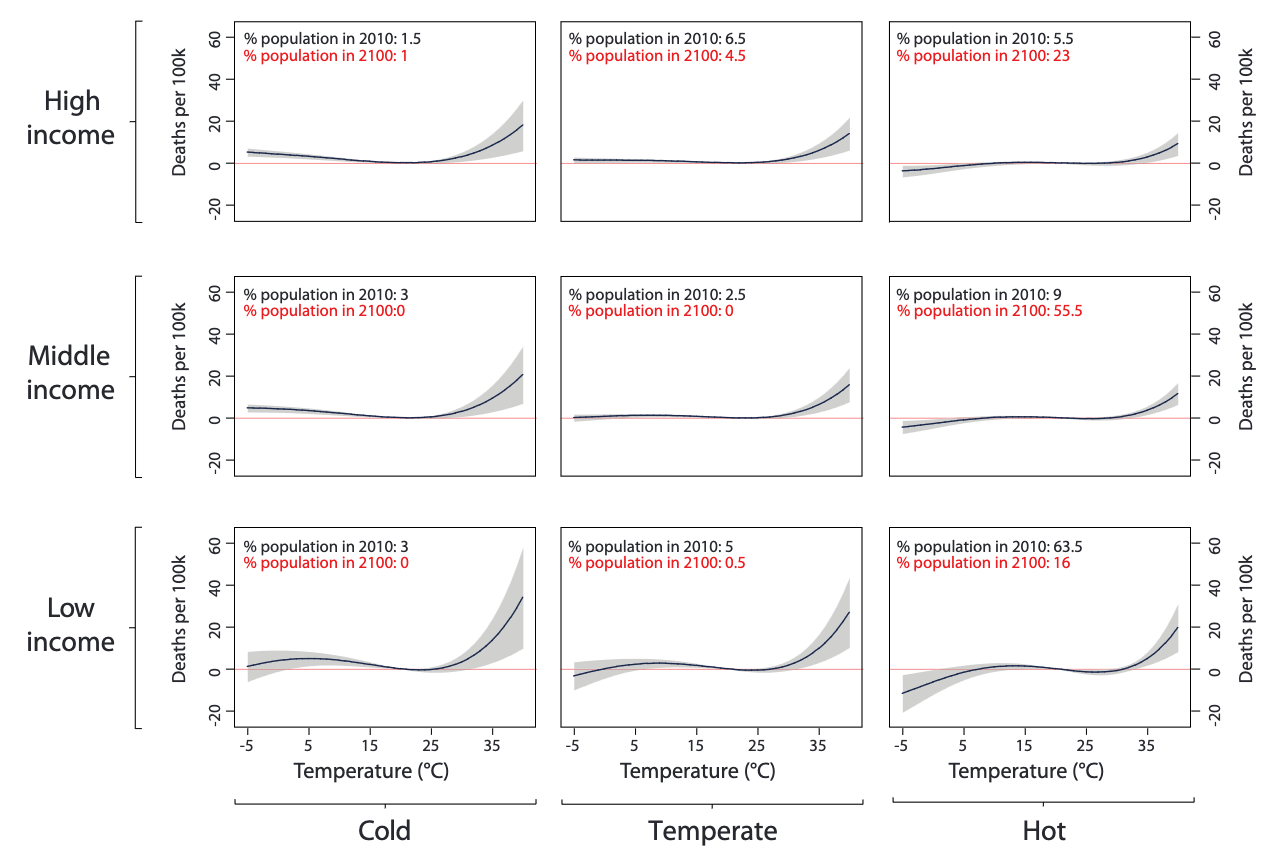
\includegraphics[width=\linewidth]{small-multiple.png}
 \caption{\label{fig:mortality_temp}Heterogeneity in the Mortality-Temperature Relationship (Age > 64 Mortality Rate) \citep[soruce:][]{carleton2022valuing}.}
\end{figure}

Figures are everything else, be it a chart graph, a photograph, a drawing, or any other illustration or non-textual depiction. In APA, any type of illustration other than a Table is referred to as a Figure. Figures are arguably the most important representations of your work. Therefore, consider the following:

\begin{tight_itemize}
\item Every figure should be of high quality. If it is not, seriously consider if it is worth including.
\item Before you include a figure, think, what value does it add to your work?
\item Figures should be centered. They must have a descriptive title that can also include copyright information or a citation.
\item Figure~\ref{fig:mortality_temp} gives the viewer the greatest number of ideas in the shortest time with the least ink in the smallest space \citep{englander2024timeless}. That is what every figure should attempt to do. This figure has nine subfigures, arranged in three rows and three columns, but because the x and y variables are the same in each subfigure, once the reader learns how to interpret one of them, they can quickly understand the others.
\item Figure~\ref{fig:mortality_temp} tells a clear narrative about the relationship between temperature, mortality, and adaptation across different income levels and climates. Subfigures are indexed by average income (rows) and climate (columns). Within a row, moving from left to right reveals how the temperature-mortality relationship compares in colder vs. hotter climates. Within a column, moving from bottom to top, shows how the temperature-mortality relationship changes as a function of income.
\item To increase your data-ink ratio, ask yourself of each figure element: can I erase this without losing clarity?
\item Use color sparingly. When using color, opt for colorblind-friendly pallettes, e.g., \texttt{viridis} in \texttt{matplotlib}.
\item According to \citet{carleton2022valuing}, a table is nearly always better than a dumb pie chart; the only worse design than a pie chart is several of them... Given their low data-density and failure to order numbers along a visual dimension, pie charts should never be used.
\end{tight_itemize}

\subsection{\label{sec:res_maths}Mathematics}

All equations appearing in your manuscript are numbered. Equations should also be looked at as a part of a sentence. It is a good practice to describe all variables, together with their units, right after the equation. An example is provided as a complete paragraph below.

According to the second law of thermodynamics, heat flows from the hot environment to the cold one as the temperature difference is equalized by diffusion. This is quantified in terms of a heat flux $\dot{q}$ in ${\rm W~m^{-2}}$ as

\begin{equation}\label{eq:conduction}
    \dot{q} = - k \frac{T_2 - T_1}{L},
\end{equation}

\noindent where $k$ is the thermal conductivity in ${\rm W~(m~K)^{-1}}$, $T_1$ is the hot environment temperature in K, $T_2$ is the cold environment temperature in K, and $L$ is the separation distance between the two environments in m.

The numbering of Eq.~(\ref{eq:conduction}) suggests that it is the first equation in Chapter~\ref{chap:res}, it is automatically assigned by \LaTeX.

According to the \href{https://www.nist.gov/pml/special-publication-811/nist-guide-si-chapter-7-rules-and-style-conventions-expressing-values}{NIST guide to the SI}, variables should be written in italic type and units in Roman type, e.g., the temperature $T_1 = 300~{\rm K}$. The above guide specifies that the expression for the value of a quantity, the unit symbol is placed after the numerical value and a space is left between the numerical value and the unit symbol. The only exceptions to this rule are for the unit symbols for degree, minute, and second for plane angle: \degree, ', and ", respectively, in which case no space is left between the numerical value and the unit symbol.

\section{\label{sec:res_lic}Licensing}

Remember, it is your responsibility to comply with the terms and conditions of the license of anything you include in your work. The very often used licenses are the variations of Creative Commons, referred to as CC, according to which you are free:

\begin{tight_itemize}
    \item to share – to copy, distribute and transmit the work,
    \item to remix – to adapt the work,
\end{tight_itemize}

under the following conditions:

\begin{tight_itemize}
    \item attribution – you must give appropriate credit, provide a link to the license, and indicate if changes were made. You may do so in any reasonable manner, but not in any way that suggests the licensor endorses you or your use.
    \item share alike – if you remix, transform, or build upon the material, you must distribute your contributions under the same or compatible license as the original.
\end{tight_itemize}

The example of how to fulfil the above conditions is provided in Figure~\ref{fig:tree}. Remember to check for license terms and conditions when using an element covered by a license. \textbf{If not license is explicitly provided, full copyright applies, therefore, you are not allowed to use a given piece of work without written consent of the author.}

\begin{figure}
 \centering
 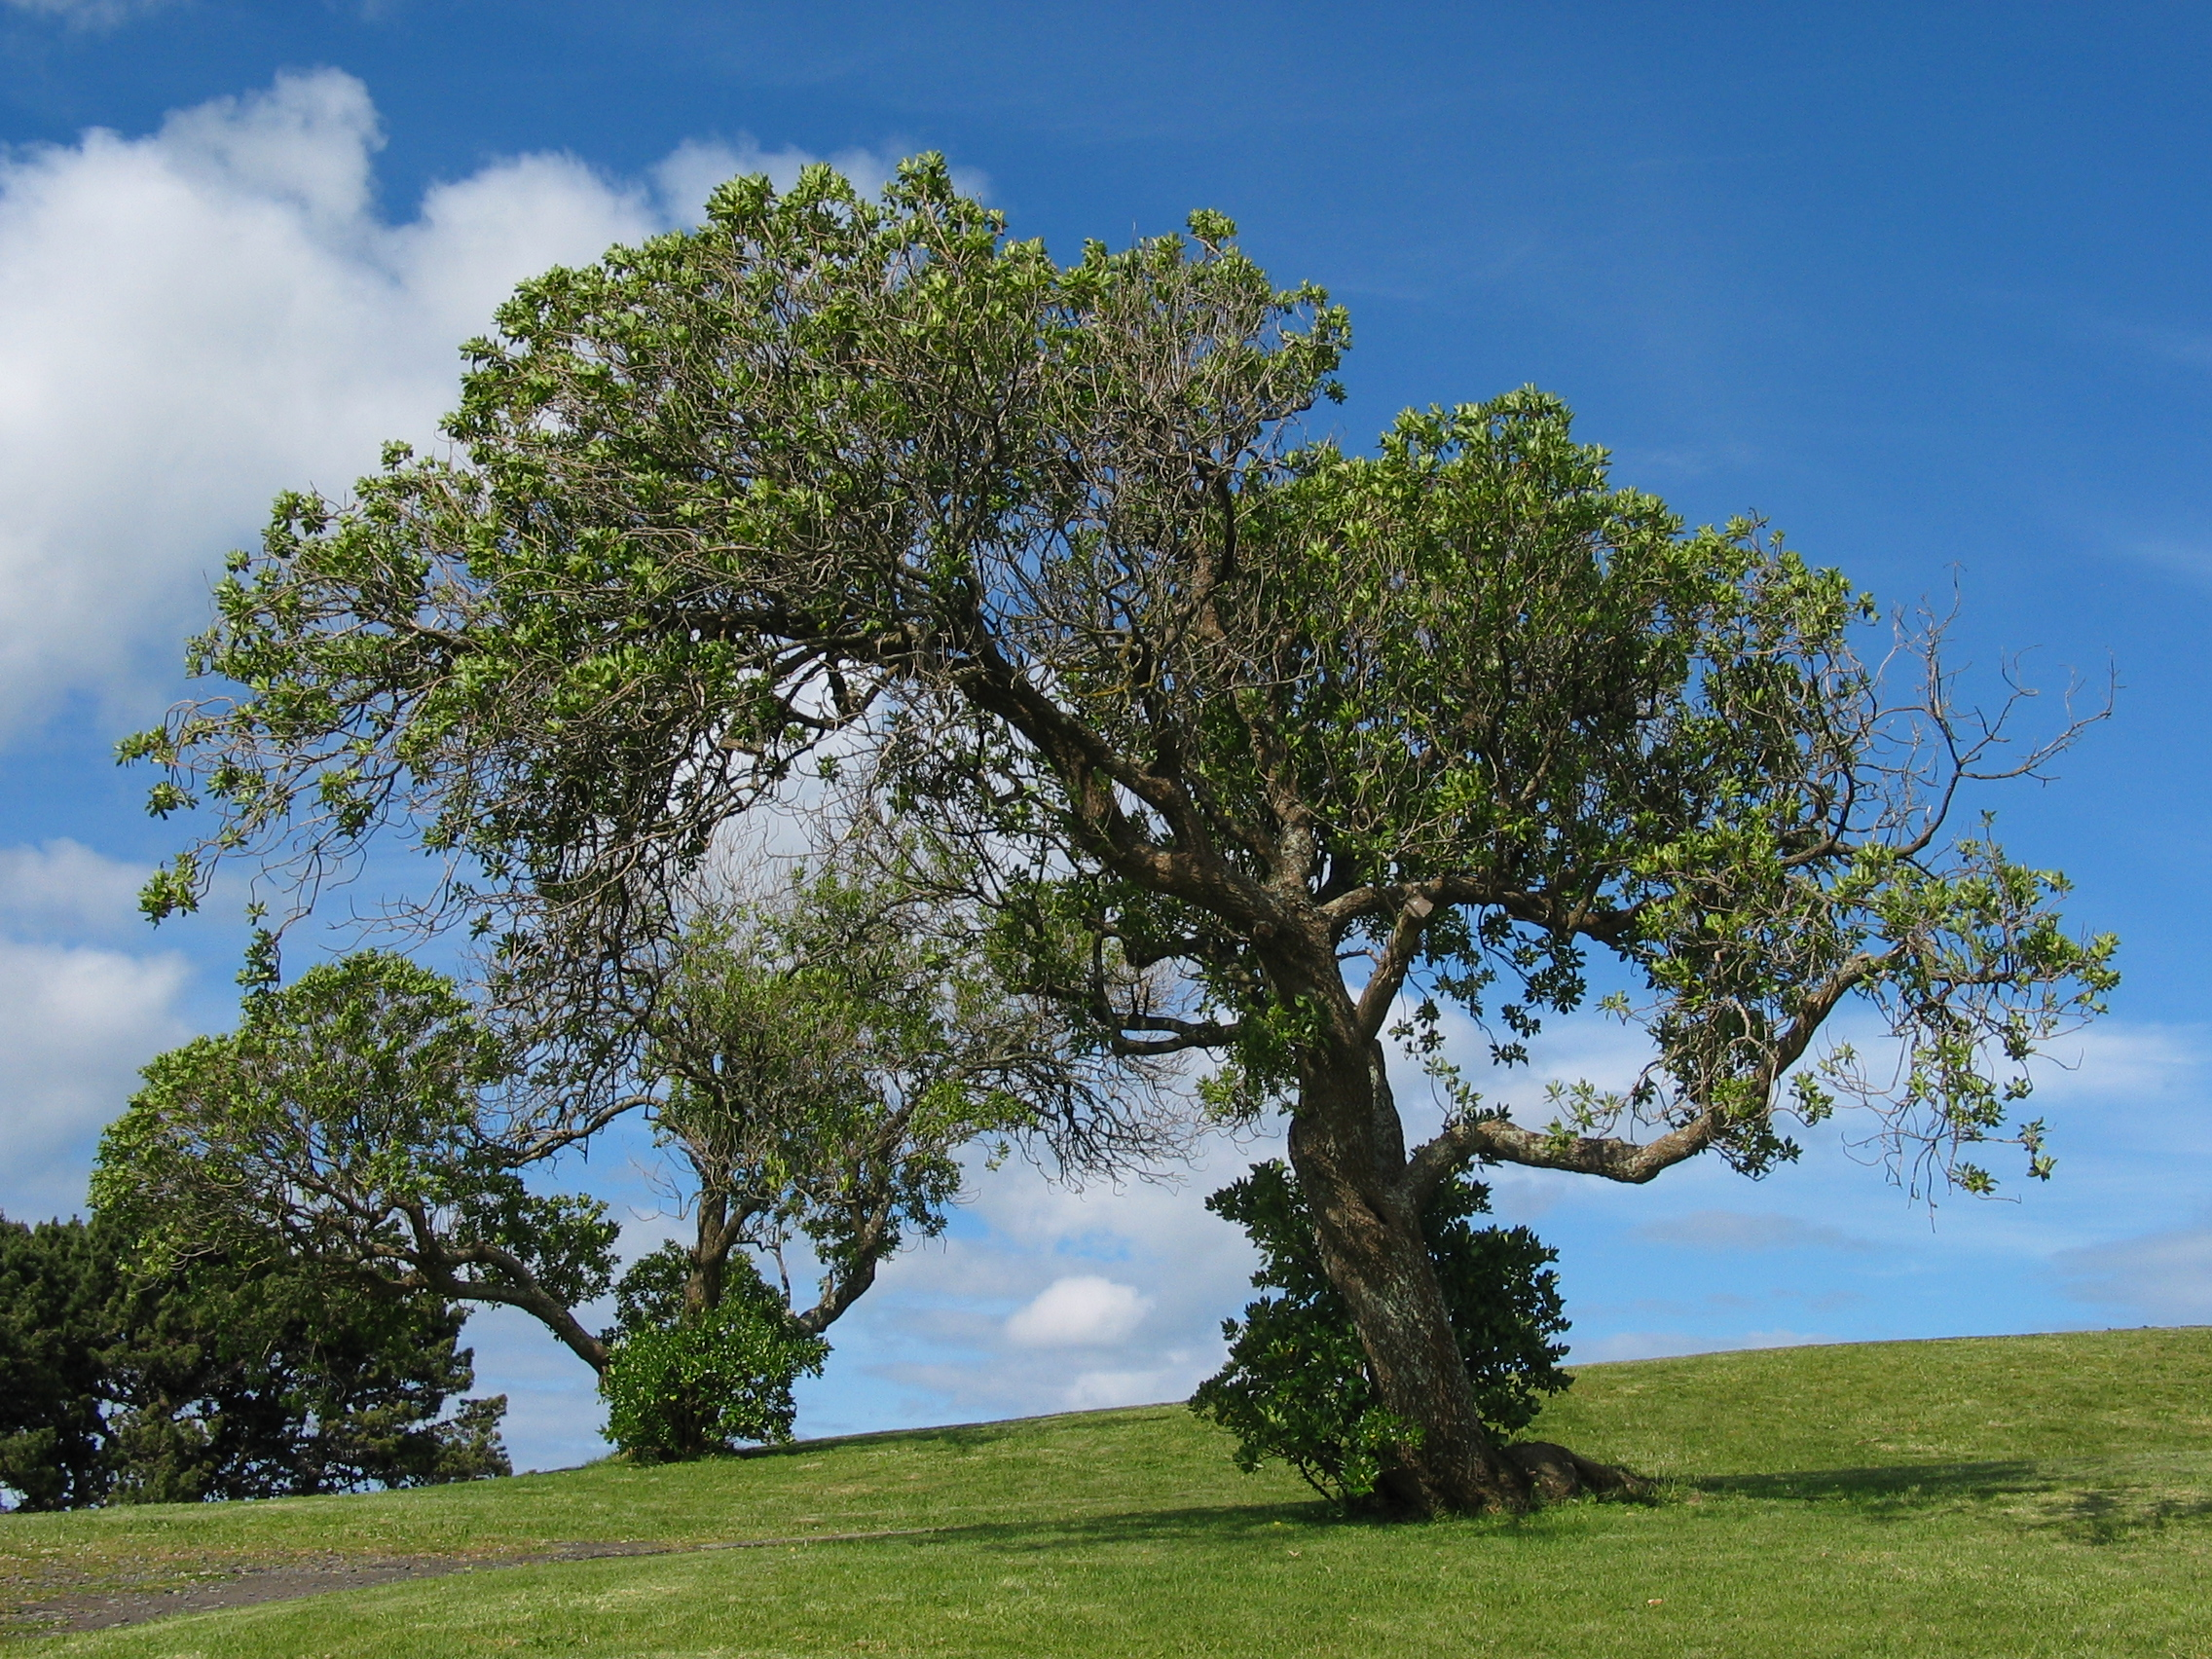
\includegraphics[width=0.6\linewidth]{Tree_example_VIS.jpg}
 \caption{\label{fig:tree}Tree on Mount Victoria Devonport, New Zealand. Image taken by \href{https://commons.wikimedia.org/wiki/User:Dschwen}{Daniel Schwen} (\href{https://creativecommons.org/licenses/by-sa/2.5/deed.en}{CC BY-SA 2.5}).}
\end{figure}

\section{\label{sec:latex}\LaTeX}

The file \texttt{main.tex} contains basic settings for the document. If you want to add a new chapter, add a line in the \texttt{main.tex} and create a new file with respective name in the \texttt{chapters} directory.

File \texttt{StyleAndSettings.sty} contains all the loaded packages and settings for formatting the document, text, figures, tables, and bibliography. Open the file, find the \texttt{hyperlink} package, and change the following lines:

\begin{verbatim}
    pdfauthor={Author},%
    pdftitle={Title},%
    pdfsubject={Bachelor Thesis/Semester Project/Master Thesis},%
    pdfkeywords={keyword1, keyword2, keyword3},%
    pdfproducer={Overleaf},%
    pdfcreator={Author},%
\end{verbatim}

\noindent so they describe your name (note that the \texttt{Author}'s name appears twice), the title of your work, the level, and the keywords. They will be embedded in the final PDF as its metadata.

\section{\label{sec:res_app}Appendices}%

You may need to use elements which distract the reader from the main plot line of your manuscript. You may also not have space because of the page limit. In either case, do not hesitate to use appendices. An appendix should appear after the bibliography, and it should contain a comprehensive set of information/drawings/tables which are helpful for the reader to understand your statements or choices more in-detail. Every appendix you add should be cited in the main matter of the manuscript, e.g., for details, see Appendix~\ref{chap:apx_exp_data}.